%% Copyright 2019-2020 Elsevier Ltd
%% 
%% This file is part of the 'CAS Bundle'.
%% --------------------------------------
%% 
%% It may be distributed under the conditions of the LaTeX Project Public
%% License, either version 1.2 of this license or (at your option) any
%% later version.  The latest version of this license is in
%%    http://www.latex-project.org/lppl.txt
%% and version 1.2 or later is part of all distributions of LaTeX
%% version 1999/12/01 or later.
%% 
%% The list of all files belonging to the 'CAS Bundle' is
%% given in the file `manifest.txt'.
%% 
%% Template article for cas-sc documentclass for 
%% double column output.

%\documentclass[a4paper,fleqn,longmktitle]{cas-sc}
\documentclass[a4paper]{cas-sc}
% \usepackage[numbers]{natbib}
\usepackage[round,sort&compress]{natbib}
\usepackage{amsmath}
\usepackage{amssymb}
\usepackage{booktabs}
% \usepackage{stfloats}
\usepackage[capitalize]{cleveref}
\usepackage{graphicx}
\usepackage{subfig}
\usepackage{enumerate} 
\usepackage{setspace}  
\usepackage{caption}
\usepackage{longtable} 
\usepackage{xcolor} 
\usepackage{tikz} 
\usepackage{tabularx}
\usepackage{enumitem}
\usepackage{bm}
\usepackage{float}
\usepackage{lineno}
\usepackage{subfig}
\usepackage{subcaption}
\usepackage{overpic}
\usepackage{soul}
\usepackage{array}
\usepackage{changepage} % 提供 adjustwidth 环境
\usepackage{ragged2e} % for \justifying
\usepackage{circuitikz}
\usepackage[usenames,dvipsnames]{pstricks}
\usepackage{pstricks-add}
\usepackage{pst-grad} % For gradients
\usepackage{pst-plot} % For axes
\usepackage{etoolbox} % For spaces in paths
\usepackage{subcaption}
\makeatletter % For spaces in paths
\patchcmd\Gread@eps{\@inputcheck#1 }{\@inputcheck"#1"\relax}{}{ }
\makeatother

\newcommand{\rlp}{\textit{RLP}}
\newcommand{\rl}{\textit{RL}\xspace}

\newcommand{\lightblue}{rgb:red,0.8;green,1;blue,1.2}
\definecolor{mygray}{rgb}{1,1,1} %
\sethlcolor{mygray} % 
\newcommand{\adj}[1]{\raisebox{-2pt}[\height][\depth]{#1}}
% Uncomment and use as if needed
%\newtheorem{theorem}{Theorem}
%\newtheorem{lemma}[theorem]{Lemma}
%\newdefinition{rmk}{Remark}
%\newproof{pf}{Proof}
%\newproof{pot}{Proof of Theorem \ref{thm}}
\setlength{\parskip}{0.2em}


% 定义柔和的蓝色
\definecolor{softblue}{RGB}{0, 102, 204}

%\newcommand{\revisedwd}[1]{{\color{softblue}\hypersetup{citecolor=softblue}
%\hypersetup{linkcolor=softblue}#1}} %\color{softblue}

\newcommand{\revisedwd}[1]{{#1}} %\color{softblue}

\captionsetup{
    justification=justified,%
}

\newenvironment{tttabular}[1]%
{\ttfamily \begin{tabular}{#1}}%
{\end{tabular}}

\begin{document}
\linenumbers
\let\WriteBookmarks\relax
\def\floatpagepagefraction{1}

% Short title
\shorttitle{}

% Main title of the paper
\title [mode = title]{3D Railway Line Detection from Multiple Images via Kalman Filter }                      
% Title footnote mark
% eg: \tnotemark[1]


% First author
%
% Options: Use if required
% eg: \author[1,3]{Author Name}[type=editor,
%       style=chinese,
%       auid=000,
%       bioid=1, 
%       prefix=Sir,
%       orcid=0000-0000-0000-0000,
%       facebook=<facebook id>,
%       twitter=<twitter id>,
%       linkedin=<linkedin id>,
%       gplus=<gplus id>]
\author[1]{Dong Wei}
\fnmark[1]
% Corresponding author indication
%\cormark[1]
% Footnote of the first author
%\fnmark[1]
% Email id of the first author
\ead{weidong@whu.edu.cn}
% Second author
\author[1]{Xiaotong Li}
\fnmark[1]
\author[1]{Yongjun Zhang}
\cormark[1]
\author[1]{Ziqian Huang}
\fnmark[1]
\ead{zhangyj@whu.edu.cn}
\author[1]{Bin Zhang}
\fnmark[1]
\author[1]{Guangshuai Wang}
\fnmark[1]
\author[1]{Xianzhang Zhu}
\fnmark[1]



% Address/affiliation
\affiliation[1]{organization={School of Remote Sensing and Information Engineering, Wuhan University},
    %addressline={Bayi Road }, 
    city={Wuhan},
    % citysep={}, % Uncomment if no comma needed between city and postcode
    postcode={430072}, 
    % state={},
    country={P.R.China}}



% Address/affiliation
\affiliation[3]{organization={College of Urban and Environmental Science, Central China Normal University},
    %addressline={Bayi Road }, 
    city={Wuhan},
    % citysep={}, % Uncomment if no comma needed between city and postcode
    postcode={430072}, 
    % state={},
    country={P.R.China}}

% Corresponding author text
\cortext[cor1]{Corresponding author}
\fntext[1]{Co-first authors. 
}

% Here goes the abstract
\begin{abstract}
Three-dimensional (3D) lines require further enhancement in both clustering and triangulation. 
Line clustering assigns multiple image lines to a single 3D line to eliminate redundant 3D lines.
Currently, it depends on a fixed and empirical parameter.
However,
a loose parameter could lead to over-clustering, 
while a strict one may cause redundant 3D lines. 
Due to the absence of ground truth, 
the assessment of line clustering remains unexplored.
Additionally, 
3D line triangulation, 
which determines the 3D line segment in object space, 
is prone to failure due to its sensitivity to positional and camera errors.

\noindent This paper aims to improve the clustering and triangulation of 3D lines and to offer a reliable evaluation method. 
(1) To achieve accurate clustering, 
we introduce a probability model,
which uses the prior error of the structure from the motion,
to determine adaptive thresholds;
\end{abstract}

% Use if graphical abstract is present
% \begin{graphicalabstract}
% \includegraphics{figs/grabs.pdf}
% \end{graphicalabstract}

% Research highlights
%\begin{highlights}
%\item Research highlights item 1
%\item Research highlights item 2
%\item Research highlights item 3
%\end{highlights}

% Keywords
% Each keyword is seperated by \sep
\begin{keywords}
    3D line segments
    \sep line clustering
    \sep line triangulation 
    \sep 3D line evaluation
\end{keywords}

\maketitle

\section{Introduction}

Currently,
the length of the railway has exceeded 1.3 million kilometers on the earth.
Thus,
extracting the center line of the rail track (CRT) accurately and efficiently, 
to support engineering design, monitor construction quality, 
and ensure operational safety,
has become one of the basic components in the maintenance of existing railways.

CRT extraction can be achieved by real-time kinematics, LiDAR,
and multiple images.
The real-time kinematic is generally mounted on a railway measurement vehicle and obtains the CRT by moving along the rail track.
In general, 
it has a satisfactory accuracy while requiring operations on the track,
thus demanding the cooperation of railway departments, 
and there are issues related to both safety and efficiency.
LiDAR sensors can be mounted on a drone, 
which is more convenient and secure than real-time kinematic. 
Because a further process, 
like point segmentation or classification,
is required for CRT extraction,
the drone must maintain a low flight altitude to satisfy the standards of the point-cloud density,
which would impact the efficiency.
A drone with cameras can capture multiple images efficiently with a safe distance from the railway area.
But CRT extraction is challenging in multiple images:
(1) The dense points reconstructed with images are inaccurate around the railway track because of the occlusion and matching problems caused by the parallax variation.
(2) Joining image semantics to obtain CRT might be workable;
However,
how to detect the semantics of CRT accurately and completely in multiple images remains to be studied.













\section{Related works}
\section{Methodology}

The flow of our methodology is presented in Figure 1.
We take aerial images of the railway area as input,
for which SfM and point clouds are used in advanced with existing software.
We first extract the image line and convert it to a space line with the locally optimal plane of the point cloud.
Then,
we cluster the single 3D line to RT candidates with the frame work derived from DBSCAN,  
during which the texture information of multiple images extracted from ResNet is used as one of the inlier distance.
Having obtained the RT cluster, 
we then trace and reconstruct the vector-based RT in the Kalman framwork,
which fully exploits the RT structure and the multi-view geometries to resolve the uncertainty caused by initial image line segment extraction and the point cloud error.
The railway-track pair is the start seed of our Kalman method.
We first convert image lines to 3D lines with the local optimal plane of the point cloud.
Then,
we cluster the single 3D line to RT pairs with DBSCAN frame work,  
during which the deep feature of multiple images is used as the inlier distance.





\subsection{Railway track with Kalman filter}

Let us first introduce the Kalman filter that optimize the \textit{RLP} without the geometry constraint between each other.
The state to be estimated is the two points and directions on the the \textit{RLP}:
\begin{equation}
\mathbf{x} = \begin{bmatrix}
    \mathbf p_1,\mathbf d_1,\mathbf p_2,\mathbf d_2 
\end{bmatrix}^ \top,
\end{equation}
where $\mathbf p_i=\left(x_i, y_i, z_i\right)$ denotes the position 
and $\mathbf d_i=\left(dx_i, dy_i, dz_i\right)$ is the normalized vector represents the direction.
Then,
the linear stochastic difference equation govern the state transition is
\begin{equation}
        \mathbf{x}_{k+1}= 
        \operatorname{diag} \left(\mathrm I,t \! \cdot \! \mathrm I, \mathrm I, t \! \cdot \! \mathrm I \right) \mathbf{x}_{k} + \mathbf{w}_k,
        \label {eq_statetransition}
\end{equation}
where $\mathrm I_{3\times3}$ is the identity matrix and $p \left(\mathbf w_k \right) \sim N(0, Q)$.
In each transition,
we can reconstruct the 3D line with multiple images (\cref*{sec_linereconstruction} ),
with which the observed position and direction related to $\mathbf x_k$ can be obtained.
Thus,
the measurement can be the same as $\mathbf x_k$,
and the general Kalman filter to track the \textit{RPL} is
\begin{equation}
    \mathbf {\hat x}_k =\mathbf {\hat x}_k^{\mbox -}+ \mathrm K\left(\mathbf z_k - \mathbf {\hat x}_k^{\mbox -}\right),\quad
    \mathbf z_k = \mathbf x_k+ \mathbf v_k,
\end{equation}
where $p \left(\mathbf v_k \right) \sim N(0, R)$,
$\mathbf {\hat x}_k^{\mbox -}$ is the prediction with \cref{eq_statetransition},
and $\mathrm K$ is the Kalman gain that iteratively calculated from the estimate error.
Please refer to (ref) for the details of Kalman gain. 

Now we add two geometry constraints of the \textit{RLP} to the filter process:
(1) $\mathbf d_1$ and $\mathbf d_2$ should be as close as possible;
and (2) The change in distance between $\mathbf p_1$ and $\mathbf p_2$ is as small as possible.


\subsection{Accurate railway line reconstruction}
\label{sec_linereconstruction}

\subsection{The seed generation for railway track}
We construct the rough 3D line based on the dense point cloud.
Given the end point $\mathbf p$ of a 2D line segment,
we randomly sample three space points around $\mathbf p$ to construct the plane $\pi$,
and we cast a ray $\mathbf r$ passing through $\mathbf p$ from the camera center.
Then,
the 3D point candidate $\mathrm P \in R ^ {3\times1}$ for $\mathbf p$ can be obtained by $\mathbf r$-to-$\pi$ intersection,
and the candidate 3D line $\mathrm L$ can be represented by the two 3D point:
\begin{equation}
    L =\left\{\textit{inter} \left(\pi,\mathbf r_1\right),\textit{inter} \left(\pi,\mathbf r_2\right)  \right\},
\end{equation}
where $\mathbf r_1$ and $\mathbf r_2$ are the rays of the two endpoints,
and \textit{inter} calculates the ray-to-plane intersection.
After random sampling of $n$ times,
we obtain a set of candidate 3D lines $\left\{ L\right\}_{i=1}^n$ and use the LMEDS algorithm,
which does not require an inlier threshold, to confirm the best 3D line for a 2D line:
\begin{equation}
    L^* = \arg\min_{L_i} \text{median} \left\{ d_{ij}\right\}_{j=1}^n ,
\end{equation}
where $d_{ij}$ is the projection distance between $L_i$ and $L_j$.  

We group two 3D lines as a RT pair based on their angle $\theta_{i,j}$,
overlap $o_{i,j}$,
and projection distance $d_{i,j}$:
\begin{equation}
   \left\{ RT= \left(L_i, L_j\right) \mid \theta_{i,j} < t_\theta, o_{i,j} > t_o, d_{i,j} \in I  \right\},
    \label{eq_geometrycons}
\end{equation}
$\theta_{i,j}$ and $o_{i,j}$are easy to choose,
e.g.,
$5^\circ$ and 60\%,
because the RT pair is parallel and highly overlapped;
while the interval $I$ needs the rough width $\omega$ between the two RT,
which can be acquired from construction standards or point clouds.
We recommend setting $I=\left[2/3\omega,4/3\omega\right]$ that uses one-third of $\omega$ as the margin of error.
Because a 3D line may satisfy \cref{eq_geometrycons} with many others,
the greedy algorithm is used to assign the candidate pair,
which uses the sum of the overlap rate as the maximum score.

We sort the RT based on their scores of the geometry alignment and select the top 10\% RT and use contextual information to further validate the RT pair.
In detail,
if the RT's central line is within $1^\circ$ and $t$ projection distance with another RT,
its score is increased by $\mathcal{N}\left(\mu, \left(t/3\right)^2\right)$.
we use the global average pooling layer in ResNet50 to describe the feature of the RT pair.
Because it has been trained on massive amounts of data and can capture texture information for classification in the absence of labels.
Also, 
we re-transform the image blocks to reduce the ambiguity caused by scale and rotation.
After extraction of RT features, 
we use DBSCAN to group them with the cosine distance,
and retain the group with the highest number as the seeds of RT.














\begin{figure}
    \centering
    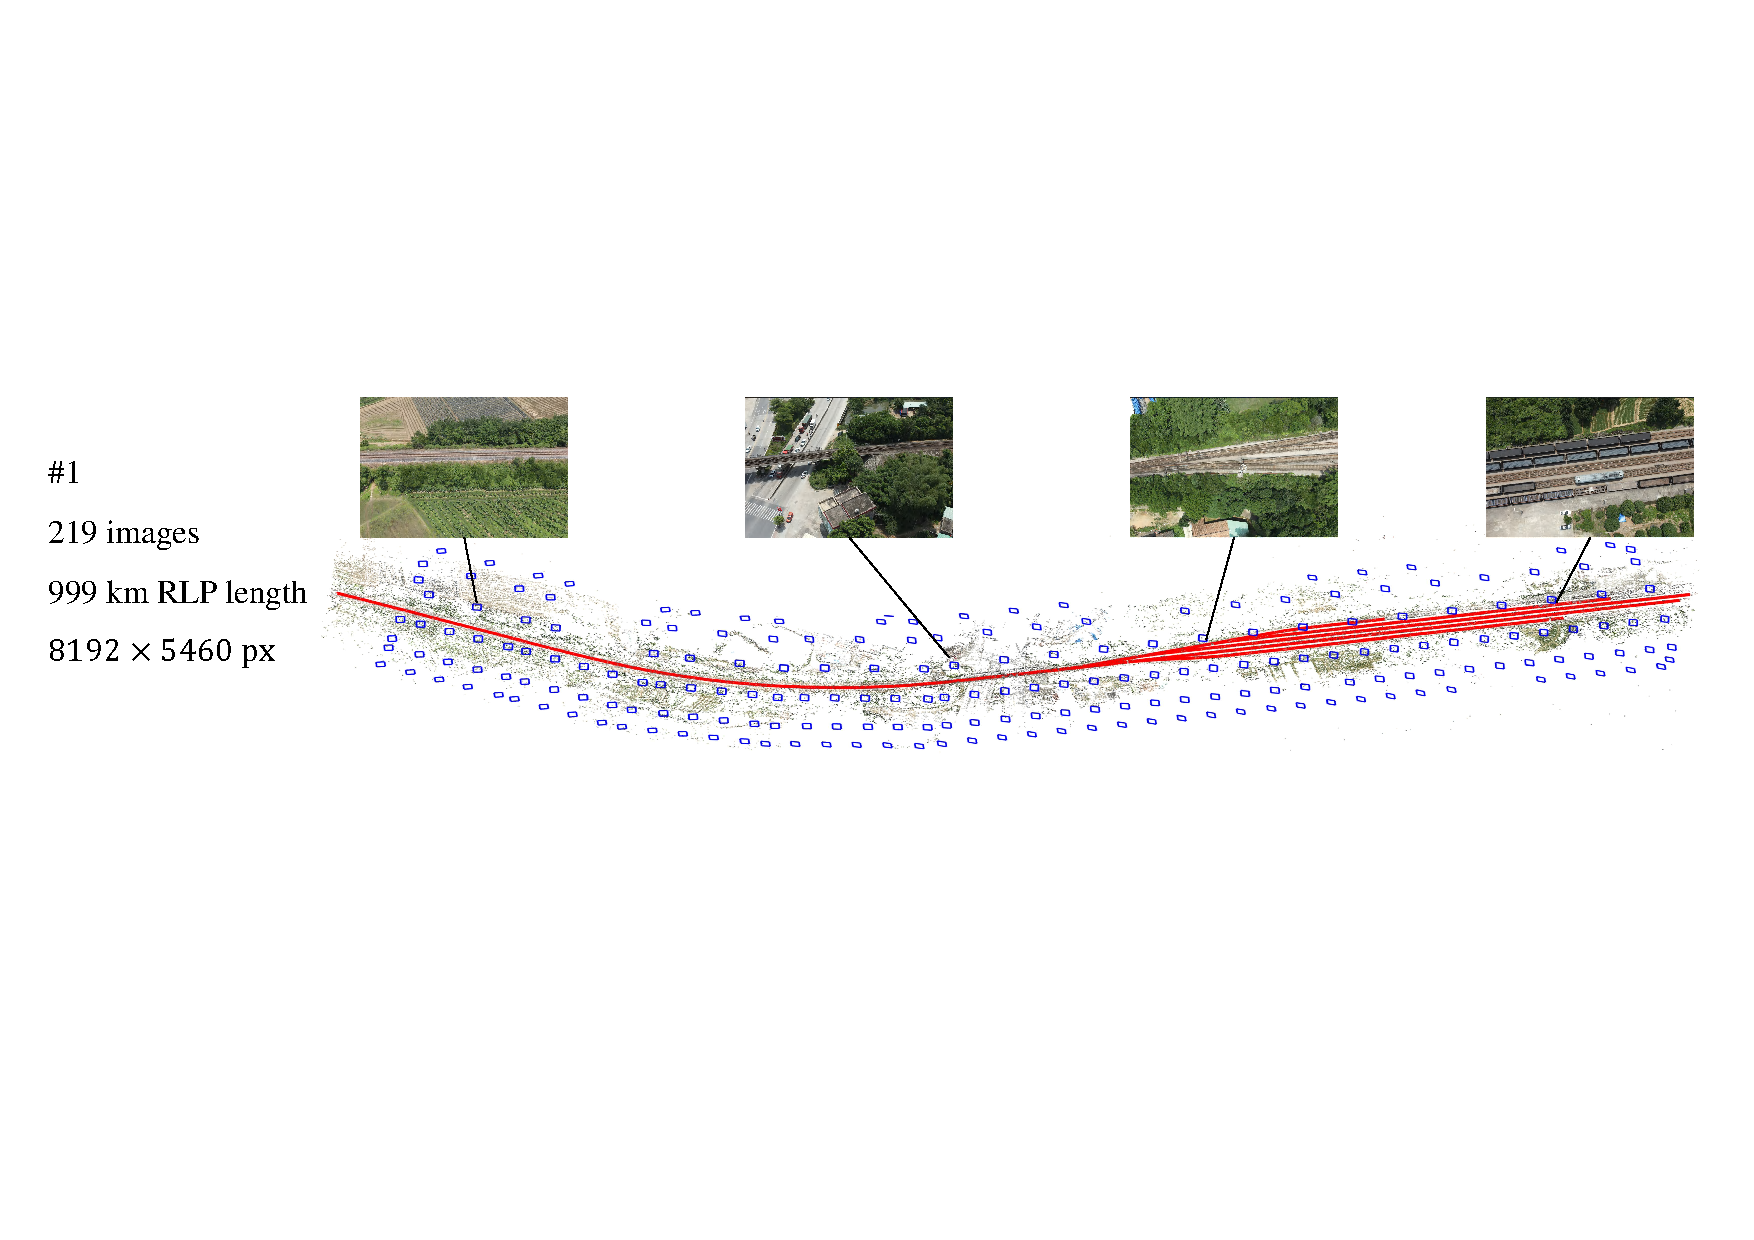
\includegraphics[width=0.95\linewidth]{images/datasets/D219.pdf}%
    \vspace{2em}
    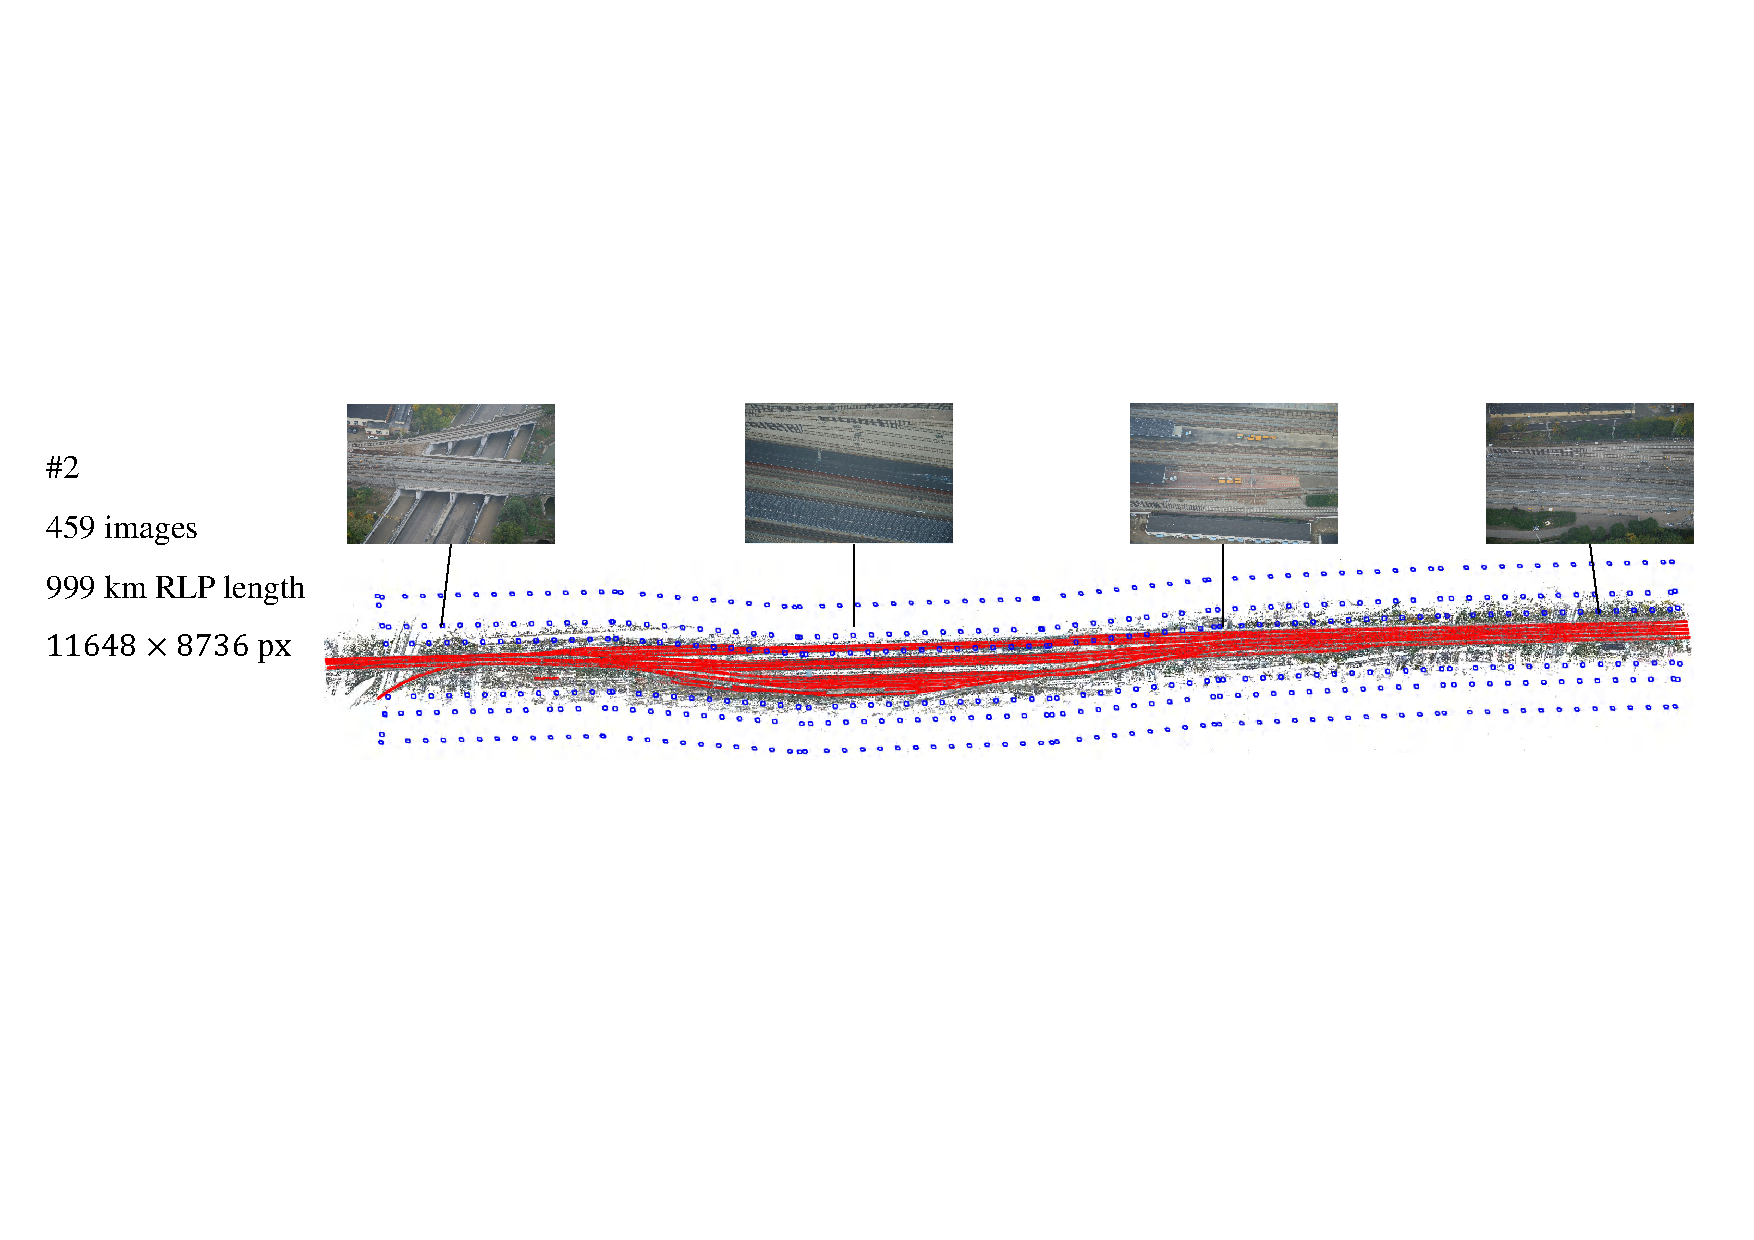
\includegraphics[width=0.95\linewidth]{images/datasets/D459.pdf}%
    \vspace{2em}
    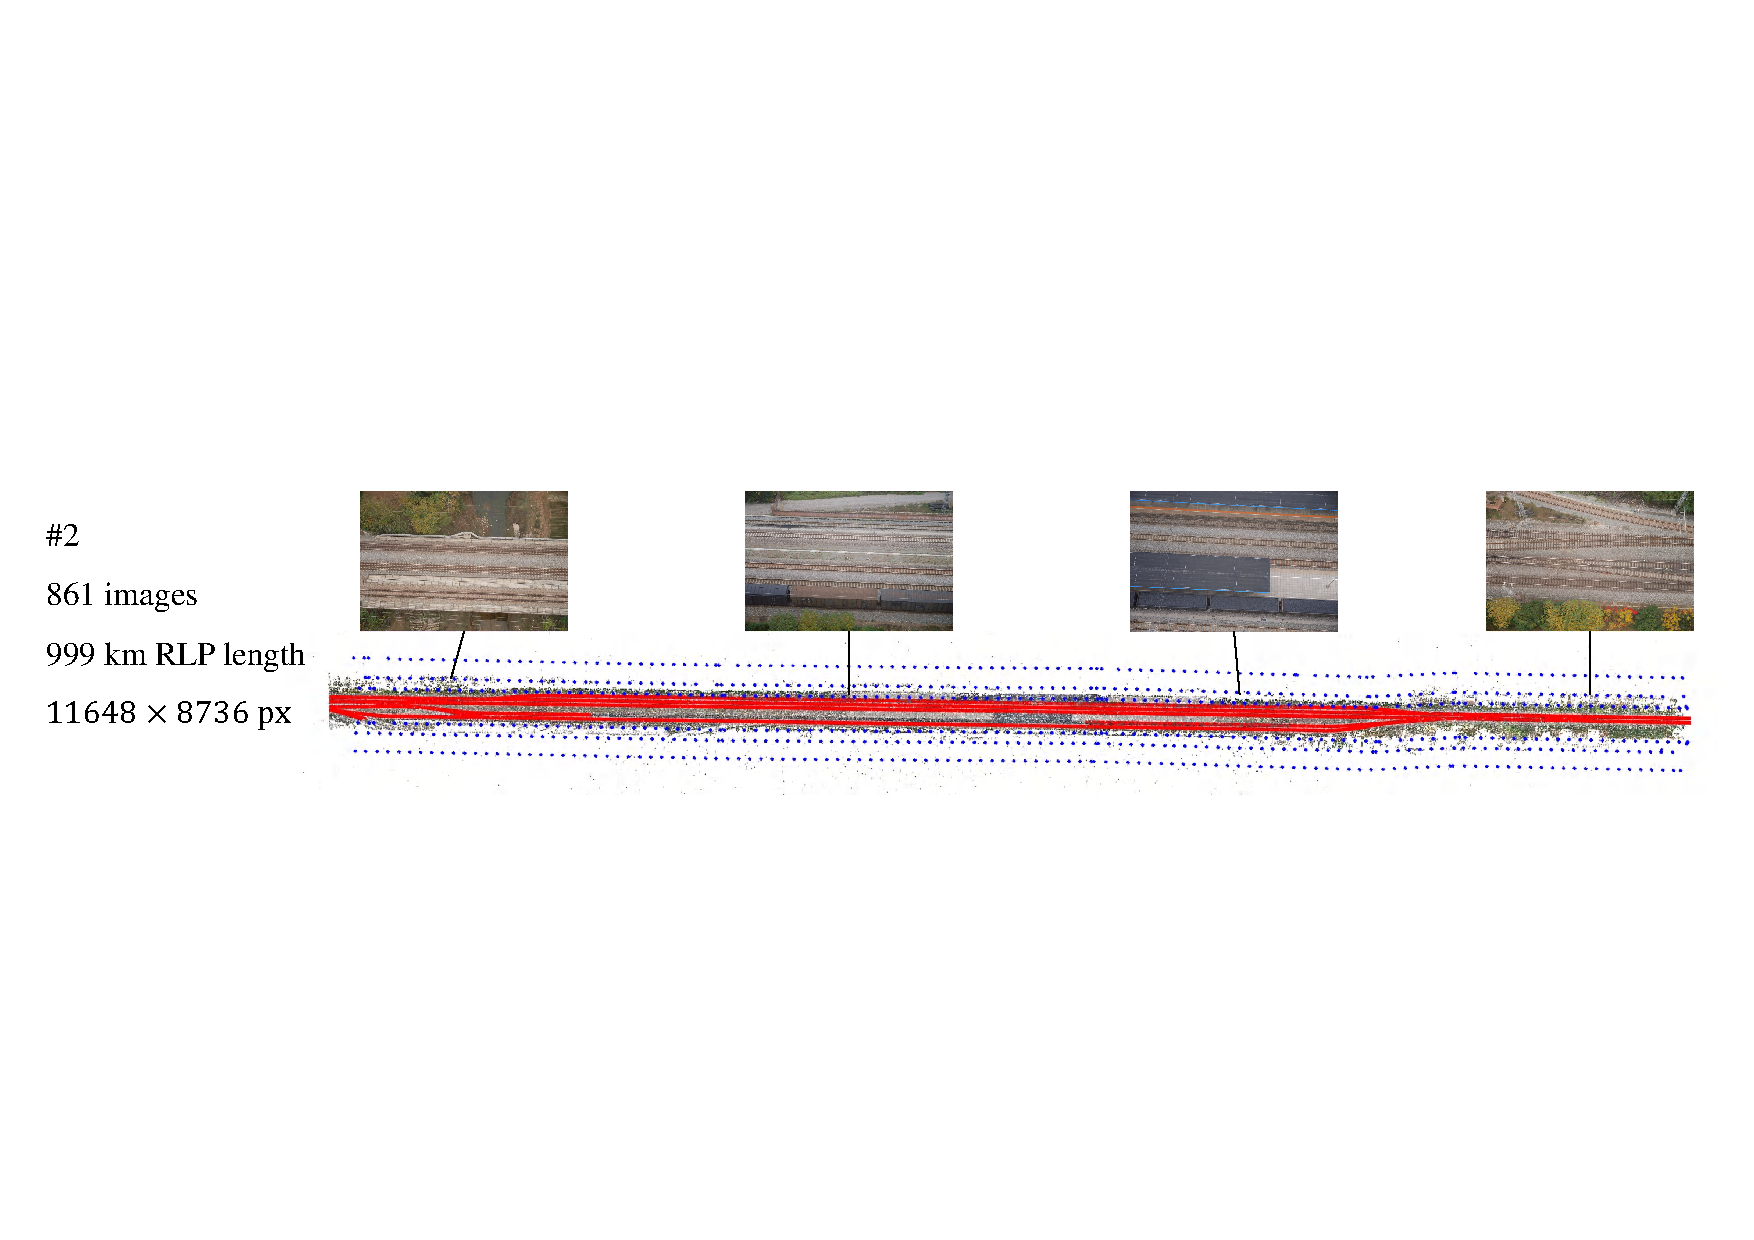
\includegraphics[width=0.95\linewidth]{images/datasets/D861.pdf}%
    \vspace{2em}
    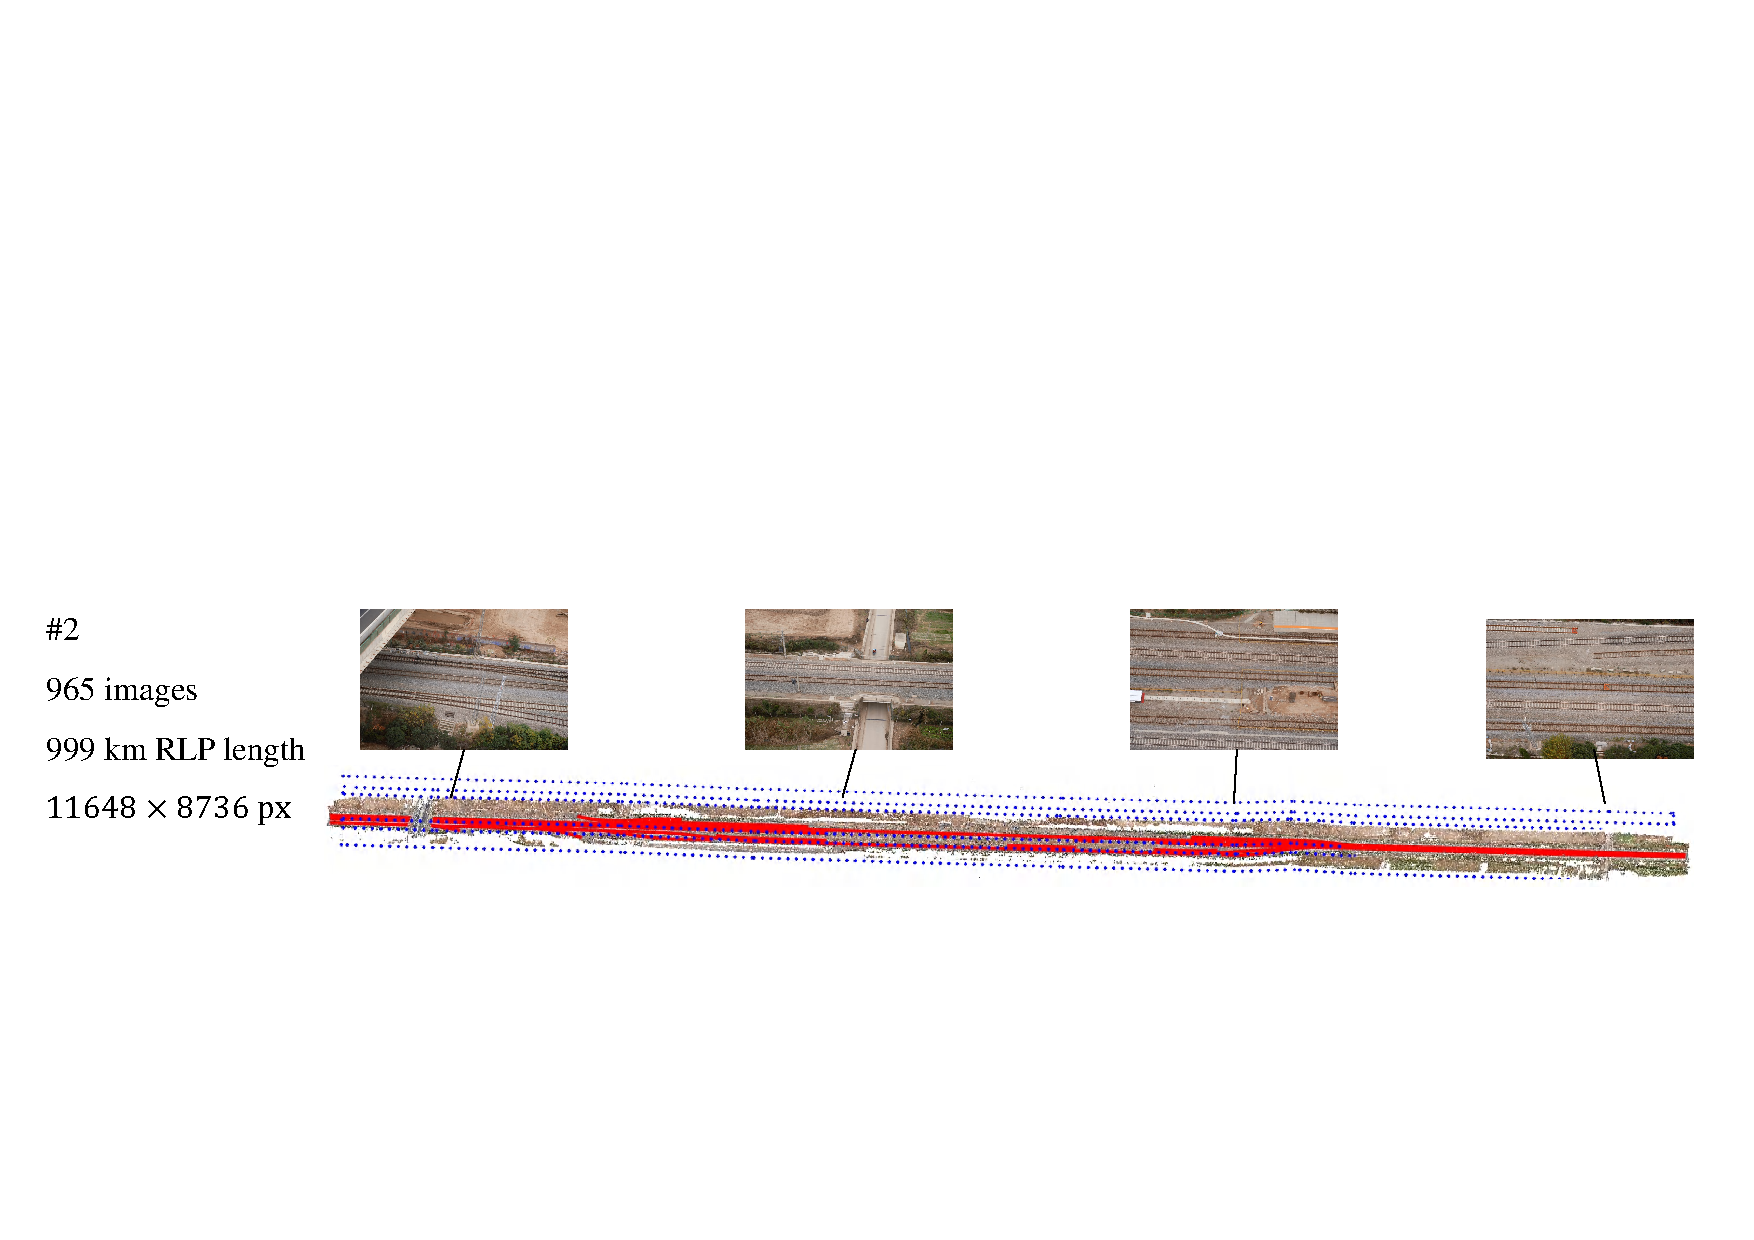
\includegraphics[width=0.95\linewidth]{images/datasets/D965.pdf}%
    \vspace{2em}
    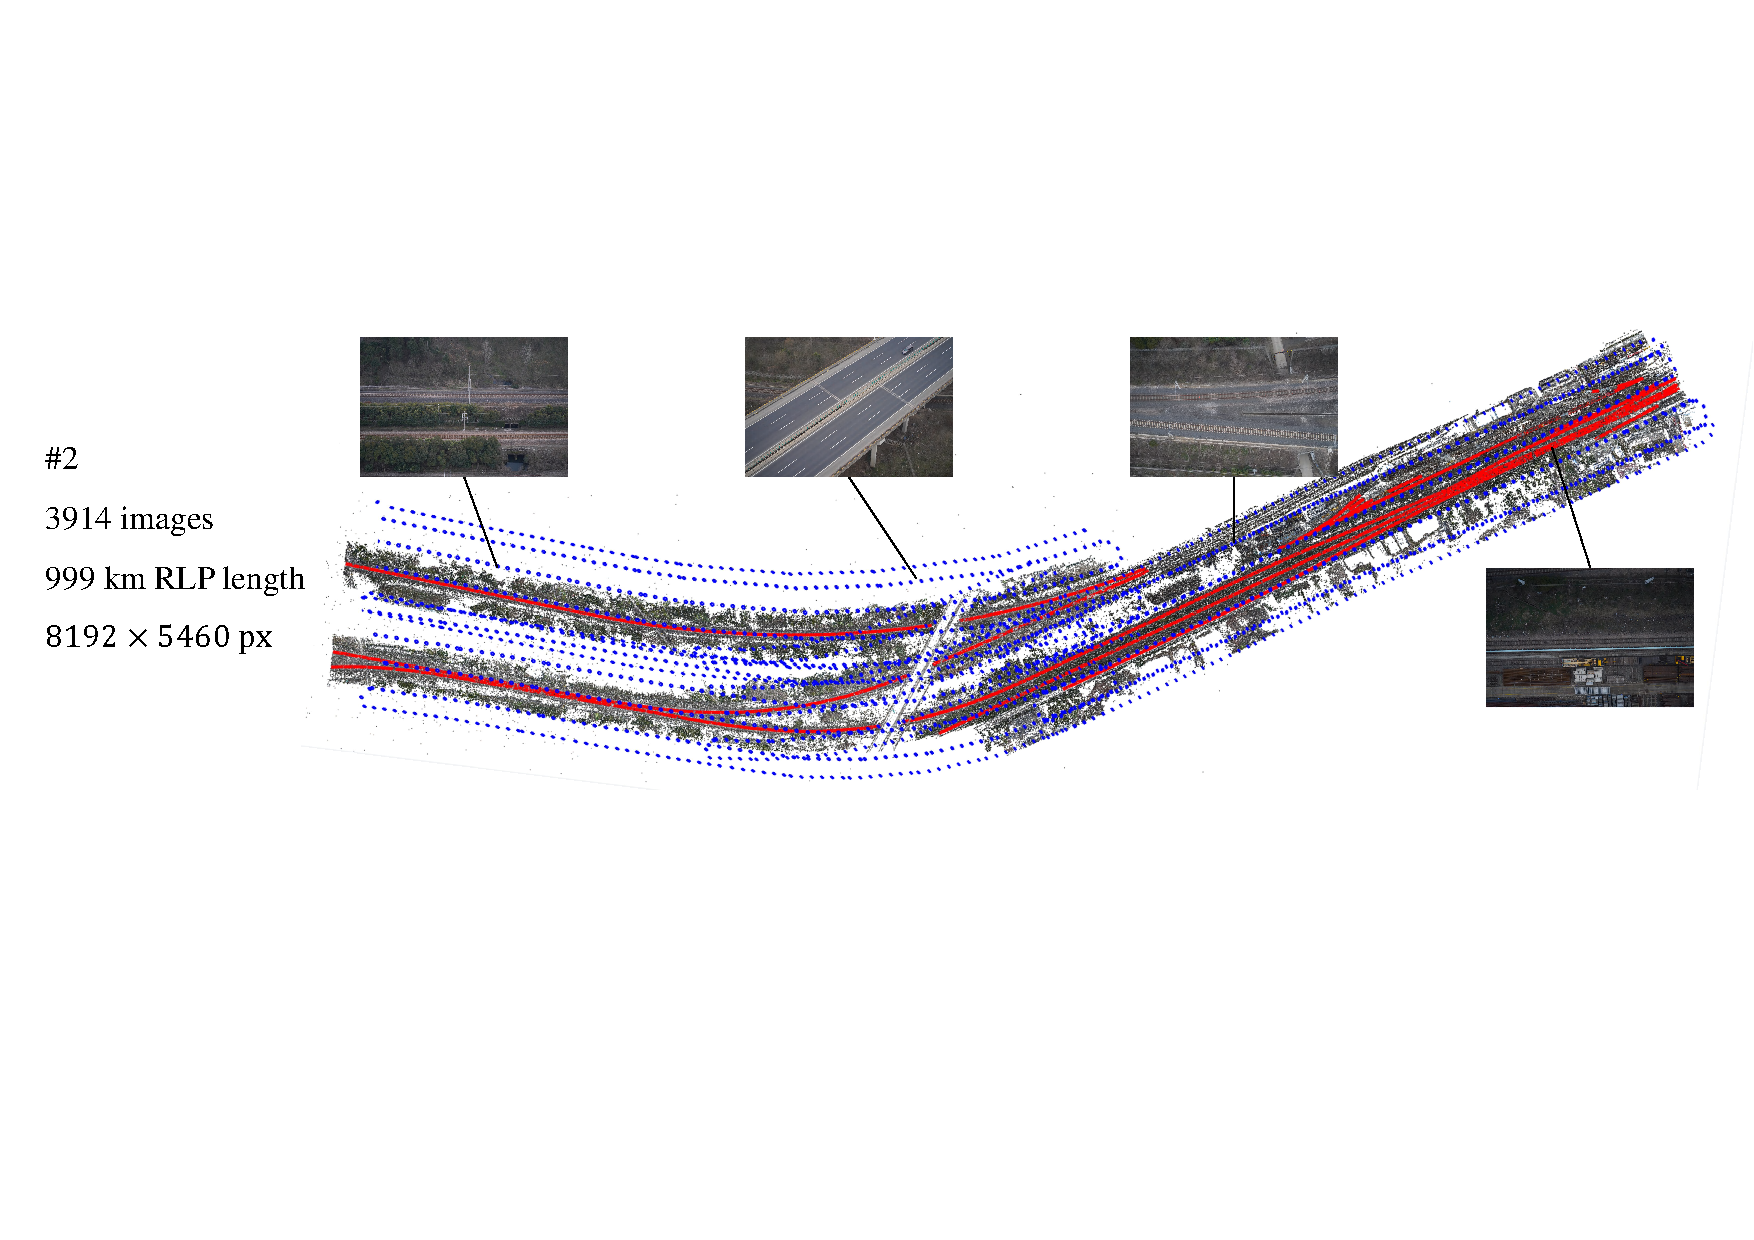
\includegraphics[width=0.95\linewidth]{images/datasets/D3914.pdf}%
    \caption{The overlook of the five datasets in the experiments,
    which are captured by drones in different provinces of China.}
    \label{fig:enter-label}
\end{figure}


\begin{figure}
    \centering
    \includegraphics[width=0.9\linewidth]{images/makegt.pdf}%
    \caption{Illustration of making the ground truth.
    We manually marked the 3D key point of the railway line on the dense point in MetaShape.}
    \label{fig:makegt}
\end{figure}

\begin{figure}
    \centering
    \subfloat[The accuracy and recall visualization]{\includegraphics[width=0.48\linewidth]{images/resvisual_1.pdf}}
    \subfloat[Visualization about the local ground truth]{\includegraphics[width=0.48\linewidth]{images/resvisual_2.pdf}}
    \caption{The visualization of the result.}
    \label{fig:resvisual}
\end{figure}

\begin{figure}
    \centering
    \subfloat[The accuracy and recall visualization]{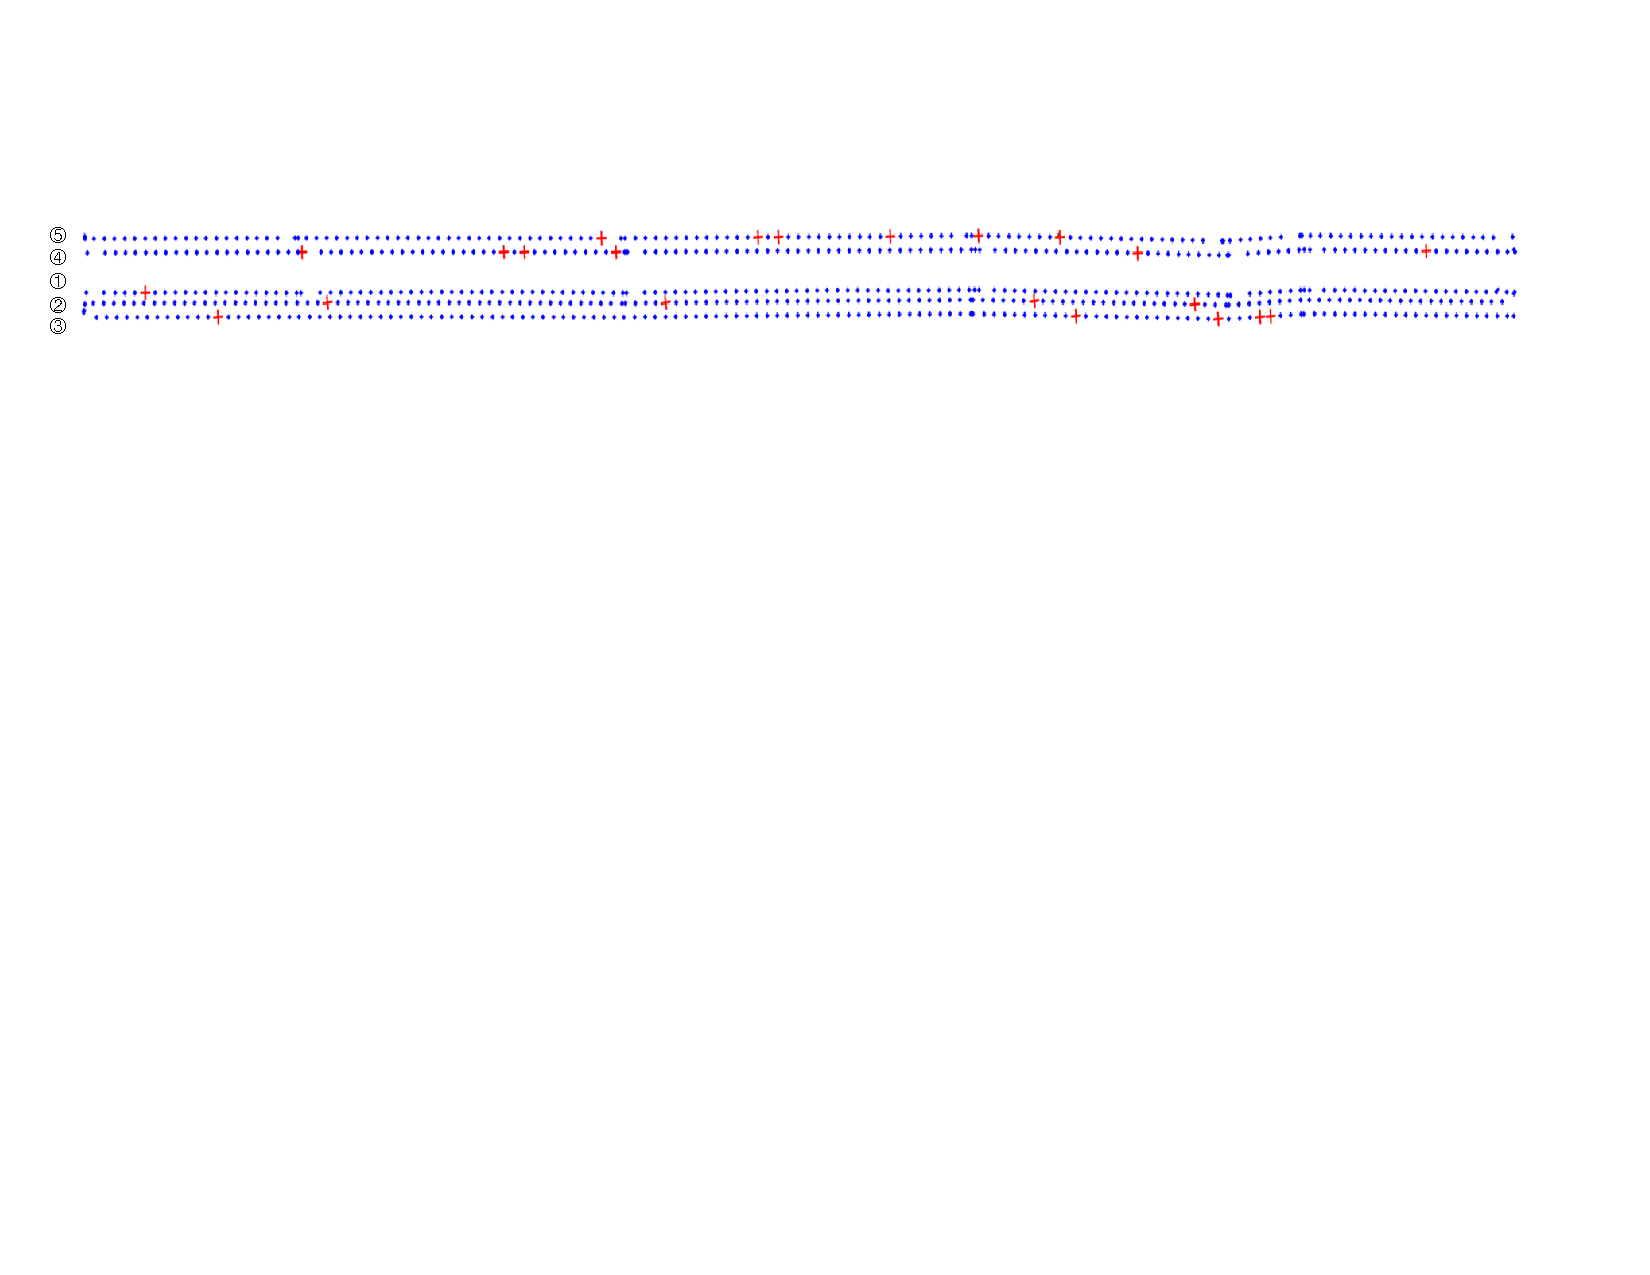
\includegraphics[width=1\linewidth]{images/imageaccuracy_1.pdf}}\\
    \subfloat[Visualization about the local ground truth]{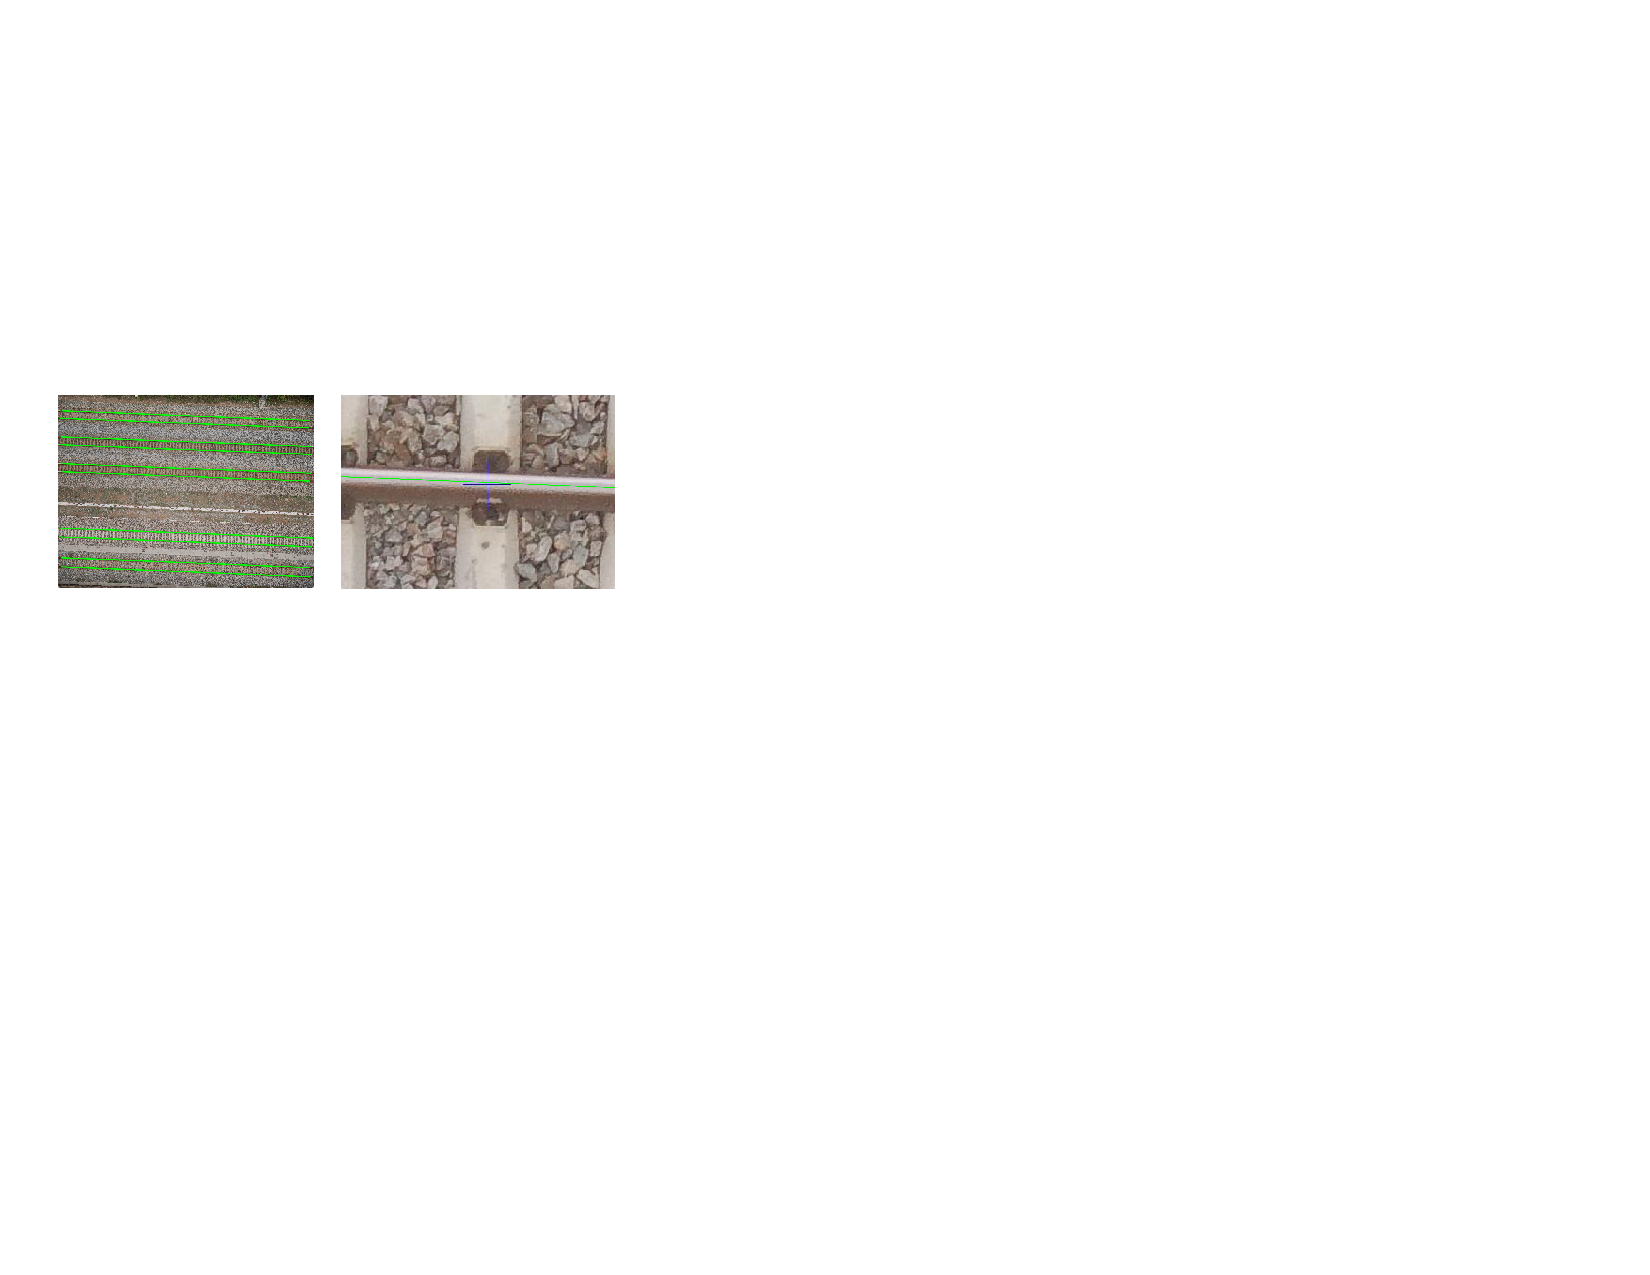
\includegraphics[width=0.46\linewidth]{images/imageaccuracy_2.pdf}}
    \subfloat[Visualization about the local ground truth]{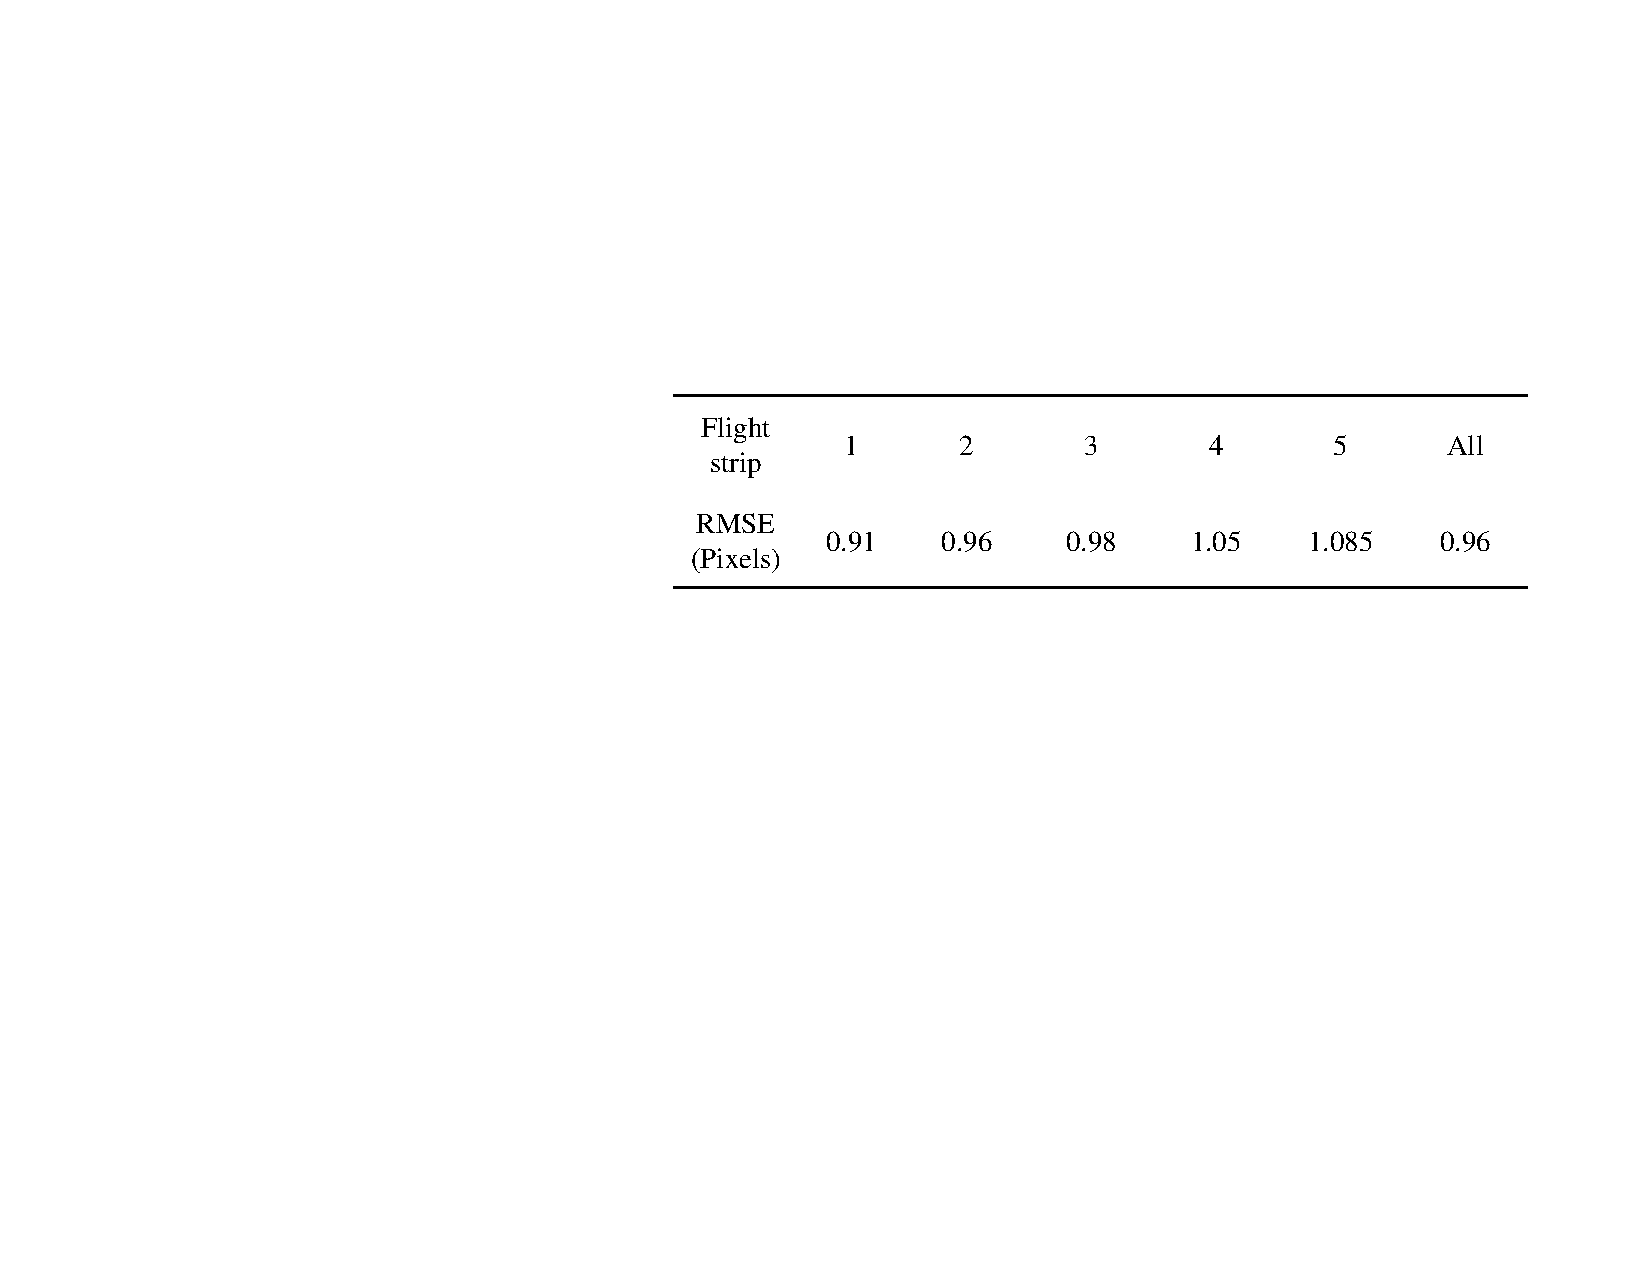
\includegraphics[width=0.5\linewidth]{images/imageaccuracy_3.pdf}}
    \caption{The visualization of the result.}
    \label{fig:resvisual}
\end{figure}

\section{Experiments}
We used five datasets to test our proposed algorithm.
The details of the data are shown in Table 1.
As shown in the figure, 
multiple-view images from two perspectives, 
one showing an aerial drone overhead operation and the other showing a vehicle operation, 
are rendered from a manually constructed 3D railway model.
We directly generate dense point clouds from the 3D model for use by other algorithms.
The other two sets of data were obtained through drones, 
and we manually drew the 3D railway track.
Currently, 
there is no publicly available code for automatically reconstructing railway segments from multi-view images. Therefore, 
we compare our approach with deep learning algorithms based on point cloud semantics.

Since our algorithm does not require training with samples,  
when compared to a 3D semantic segmentation algorithm,
it would be unfair to train a deep segmentation model and test it on the same dataset. 
Therefore, 
we use two approaches for evaluation. 
The first uses the  
The second splits a portion of the test dataset for training, 
with the remaining part used for validation.
Because the ground truth of the \textit{RL} is the vector structure,
we have to deal with the cloud segmentation result for quantitative evaluation.
As illustrated in figure.1, 
we projected the \textit{RL} cloud to the ground truth and retained the points within a distance threshold,
when the nearest two points are beyond the distance threshold, 
we say the false negative has occurred.


We use recall, accuracy, and F-score to evaluate all methods.
(1) Recall measures the ability of the method to correctly identify the true railway straight segments. 
It is the proportion of correctly identified straight segments (true positives) out of all the actual straight segments in the ground truth.
(2) Accuracy evaluates the overall correctness of the method by comparing the total number of correct predictions (both true positives and true negatives) to the total number of predictions made.
(3) F-score is the harmonic mean of precision and recall, offering a balanced measure between them. It is particularly useful when there is an uneven class distribution, giving a single metric to assess both the precision and recall of the method.





\bibliographystyle{plainnat}
\bibliography{cas-refs}


\end{document}

